\section{Mobile app implementation}
\label{sec:Mobile app implementation}
After the data collection app is implemented, the data collection process begins.
While waiting for the data set to be collected, I designed the deep model as detailed in section \ref{sec:Deep model design}.
After the design of the model is completed, the data loader and the deep model are implemented using Python programming language and TensorFlow framework.
The implementation of EfficientNet (\textit{tf.keras.applications.efficientnet.EfficientNetB0}) and the MLP classification head (\textit{tf.keras.layers.Dense} and \textit{tf.keras.layers.Dropout}) is composed directly from the TensorFlow Keras-style high-level APIs.
The Longformer implementation uses the Hugging Face Transformer\footnote{Hugging Face Transformers: \url{https://huggingface.co/transformers/}} library.
After finish implementing and training the deep model, the remaining research goal is to port the deep model to Android platform.

Although the most widely used programming language for Android development is Java, this project does not use Java except for the automatically generated initialisation codes and native function bindings.
As discussed in section \ref{sec:Framework selection}, the implementation uses React Native to develop UI and application logics.
For the parts that require high performance, such as the image pipeline, the anonymisation process, and the deep model inference process, C++ is used for multi-threaded Android native development.

\subsection{Architecture overview}
The architecture of the mobile application developed in this research is shown in Figure \ref{fig:4-mobile-arch}.
The left half of the figure describes the user interface and user interaction logic developed using React Native, and the right half describes the core functions of the application developed using C++.
These two parts use React Native Javascript Interface (JSI) for communication.

\begin{figure}[!ht]
    \centering
    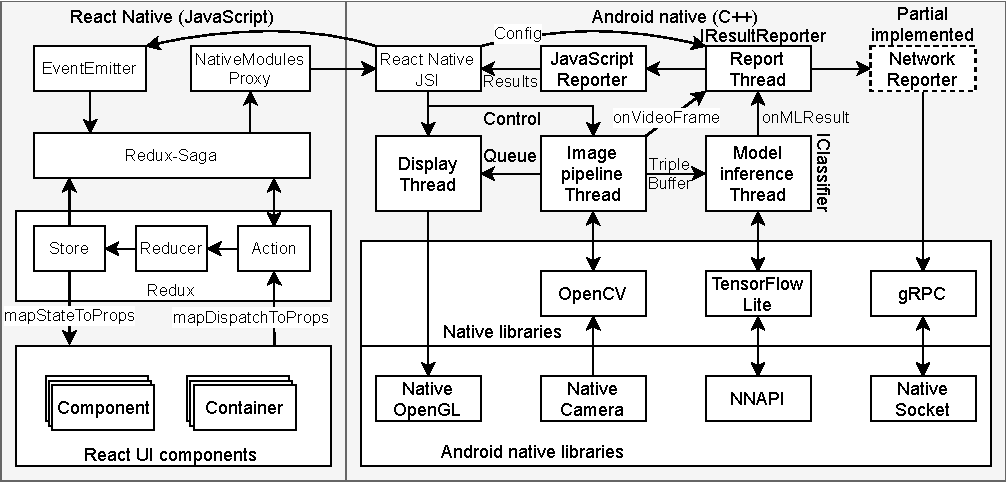
\includegraphics[width=\textwidth]{implementation/imgs/4-mobile-arch.pdf}
    \caption{Mobile app architecture and data flow}
    \label{fig:4-mobile-arch}
\end{figure}

\subsection{Tensorflow Lite adoption}

\subsection{Anonymisation with OpenCV} % 1

\begin{algorithm}[!ht]

\caption{Anonymisation procedure}
\label{algo:Anonymisation procedure}
\end{algorithm}

\subsection{Processing pipeline}

\begin{figure}[!ht]
    \centering
    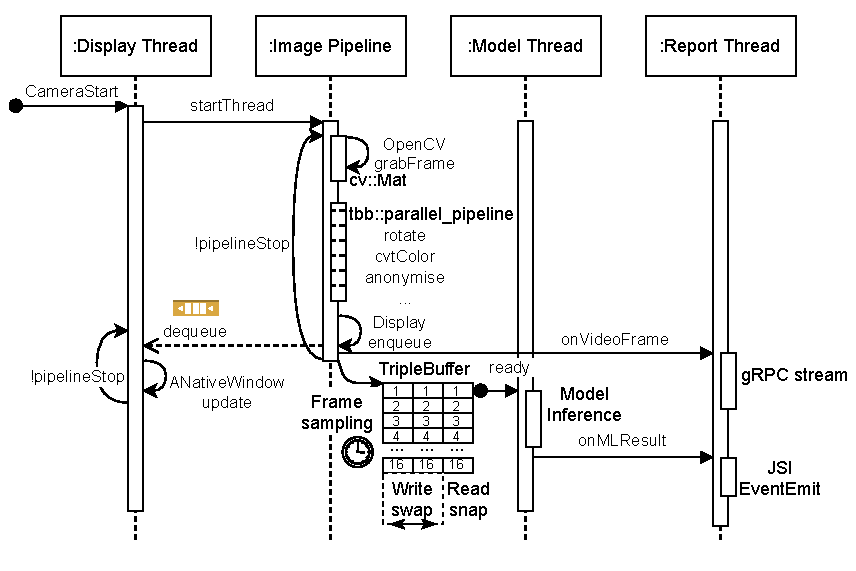
\includegraphics[width=\textwidth]{implementation/imgs/4-model-infer.pdf}
    \caption{Sequence diagram of the multi-threaded app}
    \label{fig:4-model-infer}
\end{figure}
\begin{minipage}{.5\textwidth}
\begin{algorithm}[H]

\caption{Image processing}
\label{algo:Image processing}
\end{algorithm}
\end{minipage}
\vline
\begin{minipage}{.5\textwidth}
\begin{algorithm}[H]

\caption{Model inference}
\label{algo:Model inference}
\end{algorithm}
\end{minipage}
